\documentclass[tikz,margin=1mm]{standalone}
\usetikzlibrary{calc}
%
\begin{document}
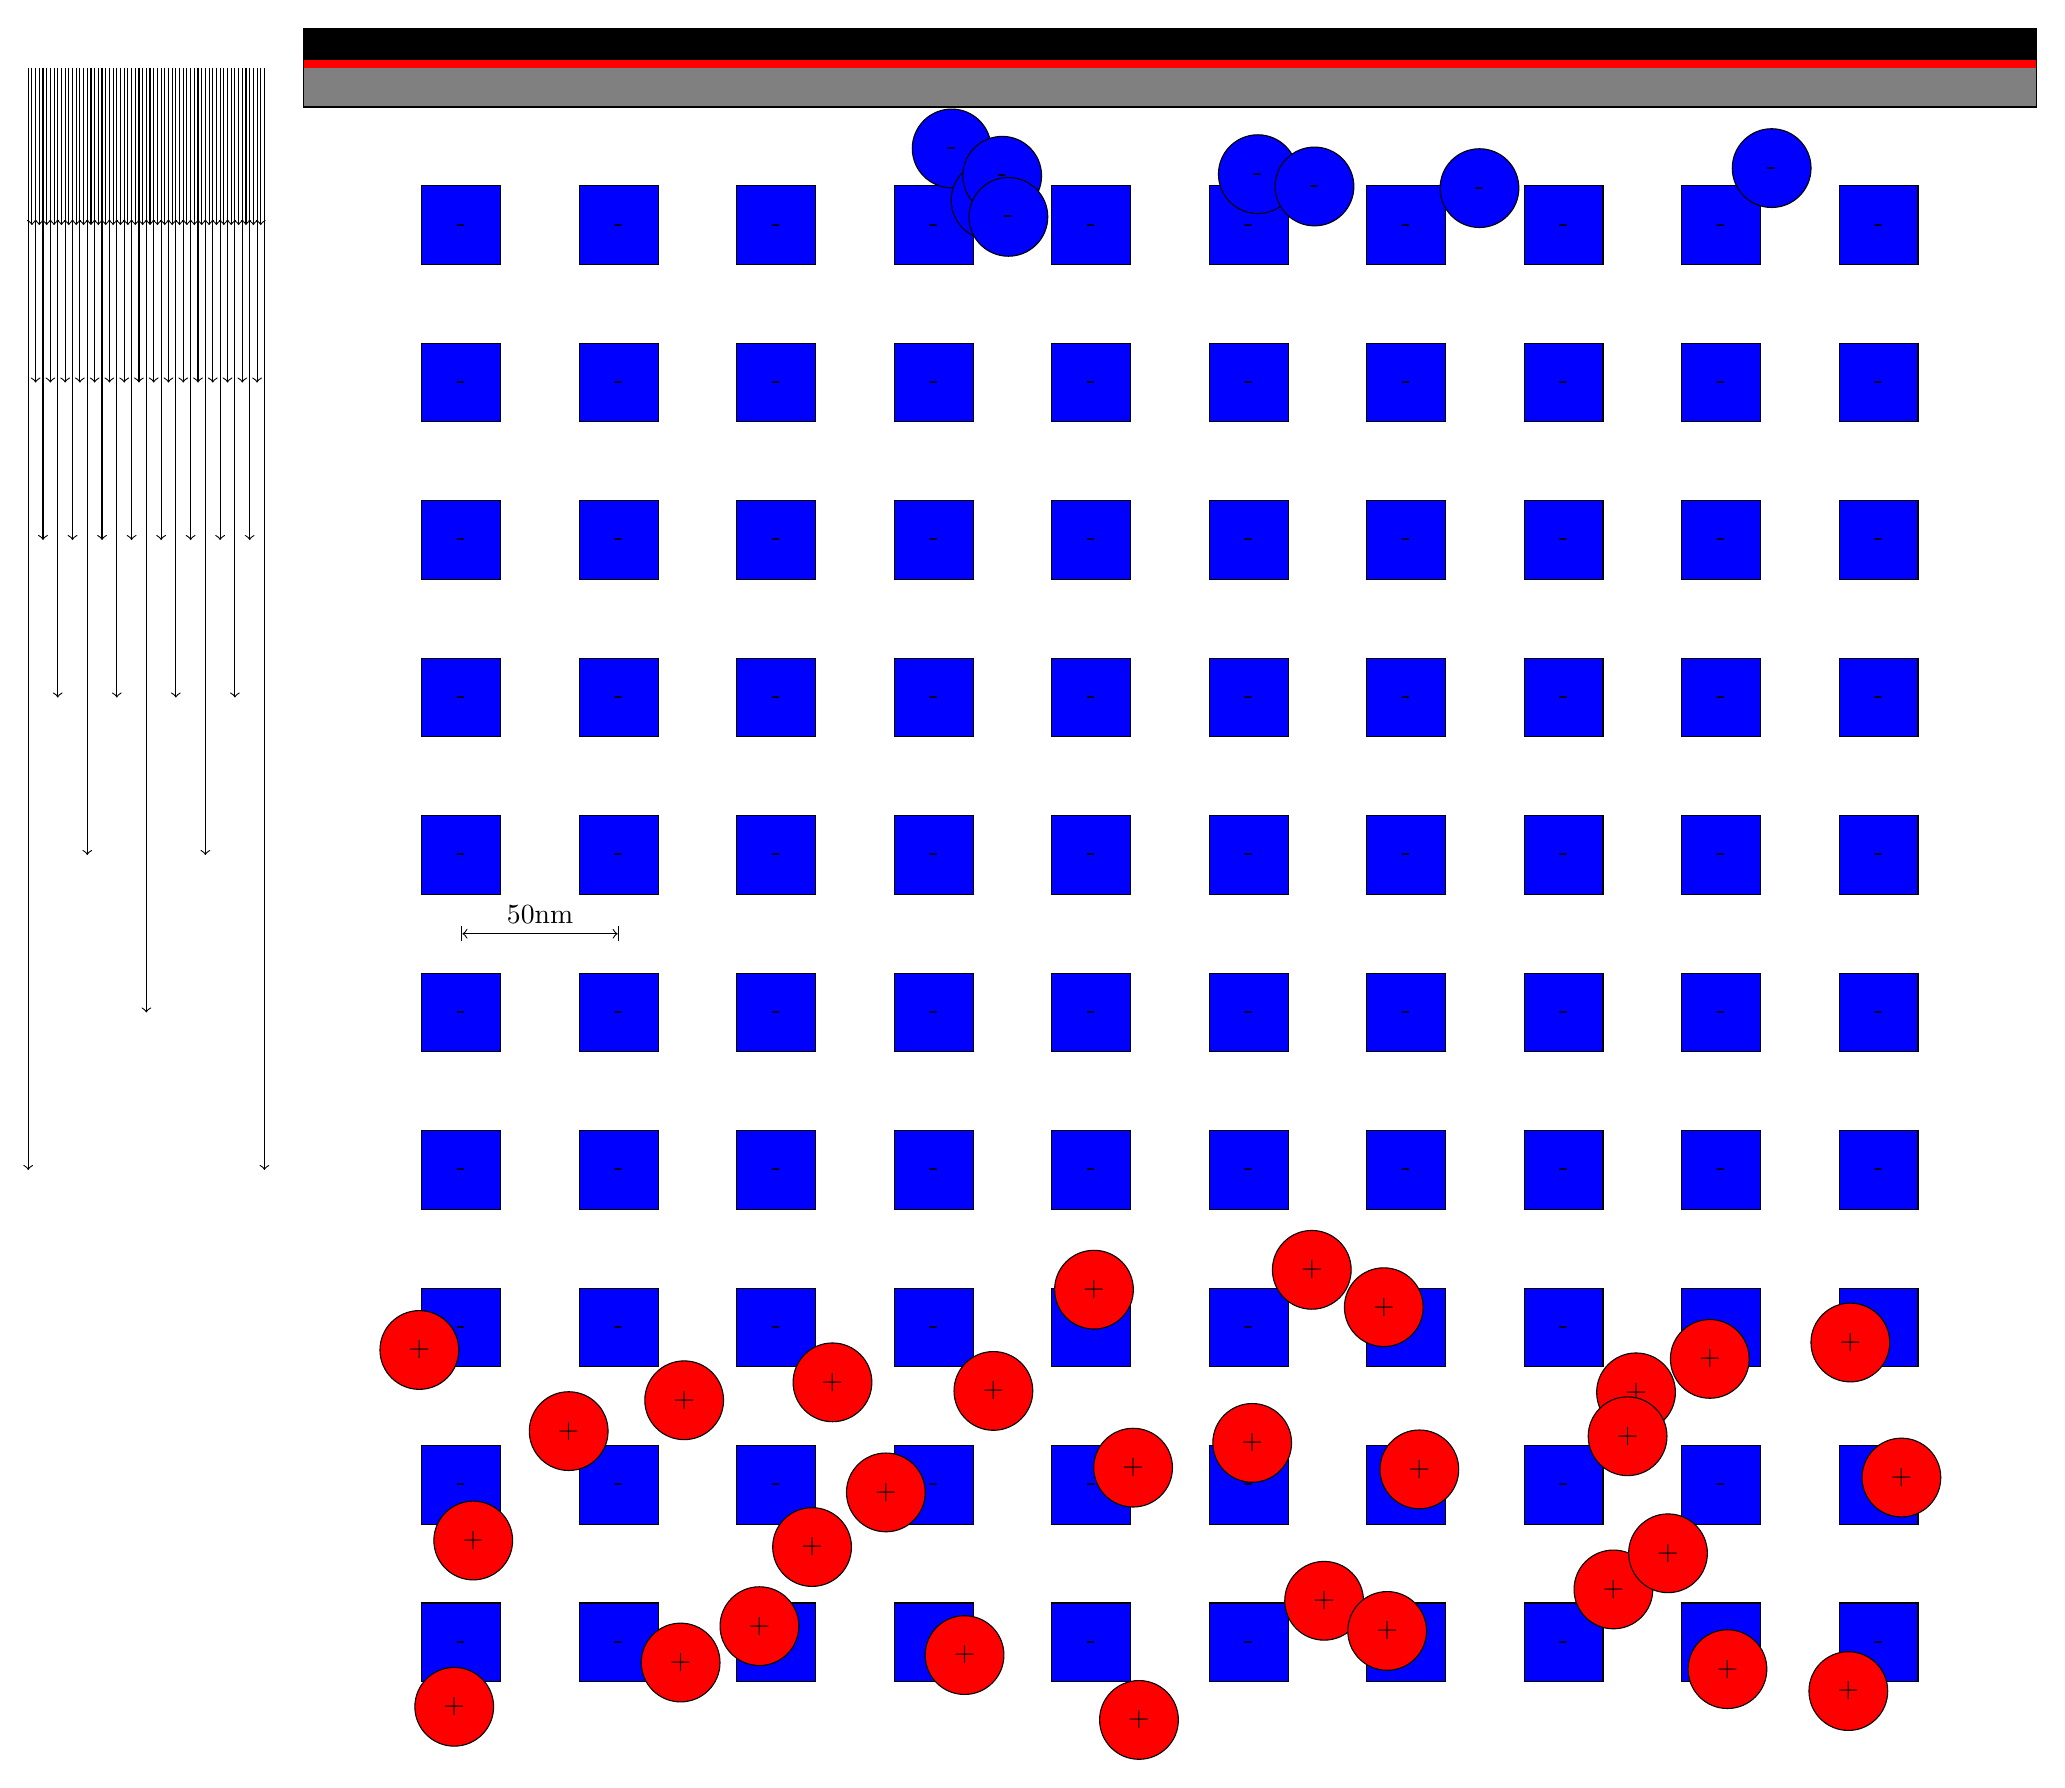
\begin{tikzpicture}
%% dopant "lattices" (simplification)
\foreach\x in {1,2,3,4,5,6,7,8,9,10}
  \foreach\y in {-1,-2,-3,-4,-5,-6,-7,-8,-9,-10}
    {
    \node[draw, minimum size=1cm, fill=blue] at (2*\x,2*\y) {-};
    }
%
\foreach\x in {1,2,3,4,5,6,7,8,9,10}
  \foreach\y in {-8,-9,-10}
    {
    \node[draw, circle, minimum size=1cm, fill=red] at ($(2*\x,2*\y) + (rand, rand)$) {+};
    }
%
\draw[fill=gray] (0, -.5) rectangle (22, 0);
% 1 cm = 50 nm (see length scale), tox ~=25 nm
\draw[fill=black] (0, 0) rectangle (22, .5);
\fill[fill=red] (0,0) rectangle (22, .1);

\foreach\x in {1,2,3,...,8}
  {
  \node[draw, circle, minimum size=1cm,fill=blue] at ($(2+9+rand*9,-2+.5*rand+.5)$) {-}; 
  }
% scale bar
\draw[|<->|] (2, -11) -- (4, -11) node[pos=0.5, above] {50nm};
%
\def\lb{-6}
\def\rb{-3}
\begin{scope}[xshift=2.5cm]
% bounds
\draw[->] (\lb, 0) -- (\lb, -14);
\draw[->] (\rb, 0) -- (\rb, -14);
% first bisection
\draw[->] (.5*\lb + .5*\rb, 0) -- (.5*\lb + .5*\rb, -12);
% second bisection
\draw[->] (.75*\lb + .25*\rb, 0) -- (.75*\lb + .25*\rb, -10);
\draw[->] (.25*\lb + .75*\rb, 0) -- (.25*\lb + .75*\rb, -10);
% third bisection
\foreach\x in {0,1,2,3}
  \draw[->] ({\lb + (\x + .5)*(\rb - \lb)/4}, 0) -- ({\lb + (\x + .5)*(\rb - \lb)/4}, -8);
% fourth bisection
\foreach\x in {0,1,2,...,7}
  \draw[->] ({\lb + (\x + .5)*(\rb - \lb)/8}, 0) -- ({\lb + (\x + .5)*(\rb - \lb)/8}, -6);
%% fifth bisection
\foreach\x in{0,1,2,...,15}
  \draw[->] ({\lb + (\x + .5)*(\rb - \lb)/16}, 0) -- ({\lb + (\x + .5)*(\rb - \lb)/16}, -4);
%% sixth bisection
\foreach\x in{0,1,2,...,31}
  \draw[->] ({\lb + (\x + .5)*(\rb - \lb)/32}, 0) -- ({\lb + (\x + .5)*(\rb - \lb)/32}, -2);
\end{scope}
%
\end{tikzpicture}
%
\end{document}
